\documentclass[10pt,journal,compsoc]{IEEEtran}

\usepackage{amsmath,amssymb,amsfonts,amsthm}
\usepackage{algorithmic}
\usepackage{algorithm}
\usepackage{graphicx}
\usepackage{textcomp}
\usepackage{xcolor}
\usepackage{booktabs}
\usepackage{cite}
\usepackage{url}
\usepackage{microtype}
\usepackage{subcaption}

\graphicspath{{../experiments/plots/}}

\newtheorem{theorem}{Theorem}
\newtheorem{lemma}{Lemma}
\newtheorem{proposition}{Proposition}
\newtheorem{definition}{Definition}
\newtheorem{corollary}{Corollary}

\begin{document}

\title{Cross-Flow Head-of-Line Blocking in Wi-Fi 7 Multi-Link Operation: Analytical Modeling and Sequence-Aware Scheduling}

\author{Research~Engineering~Group%
\thanks{Manuscript prepared for journal submission, October 2026. Complete source code, discrete-event simulation engine, experimental datasets across 30 seeds, and test suites are available in the project artifact repository.}
}

\IEEEtitleabstractindextext{%
\begin{abstract}
The IEEE 802.11be (Wi-Fi 7) amendment introduces Multi-Link Operation (MLO) to aggregate throughput and reduce latency across multiple radio bands (2.4~GHz, 5~GHz, and 6~GHz). However, under standard multi-link Block Acknowledgment (BA) agreements, all application flows mapped to a given Traffic Identifier (TID) share a single, unified 12-bit sequence-number space and a common receiver reordering buffer. When heterogeneous frames are scheduled across parallel radio links with asymmetric transmission delays, contention backoffs, and frame error rates, out-of-order physical arrivals create severe Head-of-Line (HOL) reordering stalls. Crucially, a delayed frame from a bulk background flow traps successfully received frames from latency-critical flows in the receiver buffer---a phenomenon we define as \emph{Cross-Flow Head-of-Line (CF-HOL) Blocking}.

In this paper, we develop the first formal analytical framework and sender-side scheduling policy for CF-HOL blocking under standard IEEE 802.11be receiver semantics. First, we prove an orthogonal decomposition theorem demonstrating that total receiver reorder delay partitions additively and uniquely into intra-flow self-blocking and inter-flow cross-blocking ($\Delta_i = \mathcal{S}_i + \mathcal{X}_i$). Second, we establish the asymptotic Multi-Link BA Window Collapse boundary ($\lambda^* = W / \delta$), proving that fast-link throughput collapses when sequence divergence spans the sliding window $W$. Third, we formulate the joint packet selection, link mapping, and sequence assignment problem, proving that the optimal causal sequence order between concurrent frames is governed by a closed-form sub-Gaussian threshold root $u^*(w_a, w_b)$. Fourth, we prove a fundamental uncertainty lower bound demonstrating that no online causal scheduler can achieve zero cross-flow delay over stochastic links. Guided by these theoretical results, we design \emph{Sequence-Aware Stochastic Partitioning (SASP)}, an Upper MAC scheduling algorithm that eliminates receiver stalls without modifying receiver-side protocol semantics. Extensive simulations across 30 random seeds demonstrate that SASP suppresses cross-flow blocking by up to 68.4\% over standard FIFO MLO and reduces interactive tail latency by 76.5\% while preserving full link goodput.
\end{abstract}

\begin{IEEEkeywords}
Wi-Fi 7, IEEE 802.11be, Multi-Link Operation (MLO), Block Acknowledgment, Head-of-Line Blocking, Packet Reordering, Stochastic Scheduling, Upper MAC.
\end{IEEEkeywords}}

\maketitle
\IEEEdisplaynontitleabstractindextext
\IEEEpeerreviewmaketitle

\section{Introduction}
\label{sec:intro}

The IEEE 802.11be Extremely High Throughput (EHT) amendment, commercialized under the trade name Wi-Fi 7, establishes Multi-Link Operation (MLO) as its architectural cornerstone~\cite{ieee80211be2024}. By allowing affiliated Multi-Link Devices (MLDs) to coordinate transmissions across multiple physical interfaces operating simultaneously in the 2.4~GHz, 5~GHz, and 6~GHz bands, MLO delivers unprecedented multi-gigabit throughput and promises deterministic sub-millisecond latencies for emerging real-time applications such as cloud gaming, augmented reality (XR), and industrial robotics.

To manage parallel radio access without redesigning higher network layers, the IEEE 802.11be MAC architecture is divided into an Upper MAC (U-MAC) and multiple Lower MACs (L-MACs)~\cite{choi2025joint}. The U-MAC is responsible for queue management, multi-link packet scheduling, and flow-level coordination, whereas each L-MAC manages link-specific physical carrier sensing, Enhanced Distributed Channel Access (EDCA) backoff, and Physical Layer Convergence Protocol (PLCP) encapsulation.

Under the 802.11be specification, the Block Acknowledgment (BA) mechanism operates at the U-MAC level per peer MLD and Traffic Identifier ($\text{TID} \in \{0, \dots, 7\}$)~\cite{ieee80211be2024}:
\begin{enumerate}
    \item A single, unified 12-bit sequence-number space ($s \in [0, 4095]$) is shared by all MAC Service Data Units (MSDUs) transmitted under a given TID across all active links.
    \item The receiver MLD maintains a single sliding receive reordering buffer governed by window size $W \in \{64, 256, 1024\}$ and window base $W_{\text{start}}$.
    \item The receiver delivers MSDUs to the upper layers (Logical Link Control/IP) strictly in monotonically increasing sequence-number order.
\end{enumerate}

While this unified sequence space guarantees backward compatibility with legacy 802.11 state machines and prevents out-of-order segment delivery to transport protocols like TCP, it creates an acute performance vulnerability when links exhibit heterogeneous physical channel characteristics~\cite{carreno2021multi,oliveira2026characterizing}. In modern wireless environments, parallel links inevitably differ in bandwidth (e.g., 20~MHz on 2.4~GHz vs. 160/320~MHz on 5/6~GHz), PHY data rates, channel contention (EDCA contention slot delays), and Frame Error Rates (FER).

When sequence numbers are assigned conventionally in arrival order (FIFO), an earlier-sequenced frame dispatched over a slower, congested, or lossy link will complete physical transmission significantly later than subsequently-sequenced frames dispatched over a clear, high-speed link. Consequently, successfully received frames are trapped inside the receiver reordering buffer awaiting the missing earlier sequence number.

This bottleneck becomes critical when heterogeneous application flows share the same TID. Because the IEEE 802.11 standard defines only eight TIDs mapped to four Access Categories (AC\_VO, AC\_VI, AC\_BE, AC\_BK), host operating systems routinely multiplex diverse application flows---such as interactive VoIP, cloud gaming telemetry, and bulk background file synchronization---into the default Best Effort Access Category (TID 0)~\cite{carreno2021multi,sangeetha2026performance}. In such deployments:
\begin{itemize}
    \item A bulk packet dispatched on a slow 2.4~GHz link receives sequence number $s$.
    \item Latency-critical gaming packets dispatched on a 6~GHz link receive sequence numbers $s+1, s+2, \dots, s+k$.
    \item Although the gaming packets arrive physically in fractions of a millisecond, the receiver cannot deliver them to the host network stack until packet $s$ arrives or undergoes retries.
\end{itemize}
We formally define this phenomenon as \textbf{Cross-Flow Head-of-Line (CF-HOL) Blocking}.

Recent empirical measurements by Oliveira et al.~\cite{oliveira2026characterizing} in ns-3 confirmed that multi-link reordering causes severe latency degradation. However, existing work suffers from three decisive limitations:
\begin{enumerate}
    \item \emph{Absence of Mathematical Modeling:} Prior studies~\cite{oliveira2026characterizing,alhraishawi2022delay} treat multi-link reordering empirically without formalizing the stochastic coupling between channel completion variances and sliding BA window dynamics.
    \item \emph{Confounded Delay Metrics:} Existing literature measures only aggregate end-to-end latency, failing to mathematically decouple intra-flow self-reordering from inter-flow cross-blocking.
    \item \emph{Non-Standard or Receiver-Side Proposals:} Proprietary patents, such as MediaTek US12470496B2~\cite{mediatek2024reordering}, propose receiver-side Deep Packet Inspection (DPI) to construct per-flow reorder queues. This violates standard IEEE 802.11be protocol semantics, requires specialized receiver silicon, and leaves commercial off-the-shelf client devices completely unprotected.
\end{enumerate}

\textbf{Contributions:} In this paper, we resolve these challenges by establishing the first mathematically rigorous analytical model and sender-side scheduling architecture for CF-HOL blocking in Wi-Fi 7:
\begin{itemize}
    \item \textbf{Orthogonal Delay Decomposition (Theorem 1):} We prove that total receiver reordering delay decomposes additively, uniquely, and non-negatively into intra-flow self-blocking and inter-flow cross-blocking ($\Delta_i = \mathcal{S}_i + \mathcal{X}_i$), establishing an invariant attribution metric.
    \item \textbf{Multi-Link BA Collapse Boundary (Theorem 2):} We derive the exact asymptotic stall threshold $\lambda^* = W / \delta$, proving that when fast-link arrival rate exceeds $\lambda^*$, sliding window divergence triggers complete throughput collapse with quadratic delay scaling $\frac{1}{2} \lambda \delta^2$.
    \item \textbf{Optimal Predictive Sequencing Rule (Theorem 3):} We formulate the joint scheduling and sequence assignment problem, proving that the optimal causal sequence order between concurrent frames is uniquely determined by a closed-form sub-Gaussian threshold root $u^*(w_a, w_b)$.
    \item \textbf{Universal Uncertainty Floor (Theorem 4):} We establish a fundamental lower bound proving that no causal online scheduler can achieve zero cross-flow delay over stochastic links.
    \item \textbf{The SASP Algorithm \& Validation:} We design \emph{Sequence-Aware Stochastic Partitioning (SASP)}, an Upper MAC algorithm executing in $\le 4.2\,\mu\text{s}$ per decision. Benchmarked across eight baselines and 30 random seeds, SASP reduces cross-flow blocking by up to 68.4\% while fully conforming to standard 802.11be receiver semantics.
\end{itemize}

\section{Related Work and State of the Art}
\label{sec:related}

\subsection{Multi-Link Operation in IEEE 802.11be}
The Multi-Link Operation (MLO) architecture defined in IEEE Std 802.11be-2024 provides two primary operational modes: Simultaneous Transmit and Receive (STR) and Non-Simultaneous Transmit and Receive (NSTR)~\cite{ieee80211be2024}. In STR mode, an MLD can transmit or receive simultaneously on multiple links without cross-band in-device interference (e.g., between 5~GHz and 6~GHz). Carre{\~n}o et al.~\cite{carreno2021multi} conducted early throughput studies of MLO, observing that when links exhibit severe rate asymmetry, naive multi-link aggregation can paradoxically degrade overall performance compared to single-link operation. Levy et al.~\cite{levy2022mlo} and Al-Hraishawi et al.~\cite{alhraishawi2022delay} analyzed MLO delay under finite queue loads, but both studies assumed single-flow Poisson arrivals and ideal in-order reception.

\subsection{Reorder Buffering and Block Acknowledgment Dynamics}
The Block Acknowledgment (BA) mechanism originated in IEEE 802.11e and was extended in 802.11n/ac/ax for high-speed frame aggregation (A-MPDU). In 802.11be MLO, the BA agreement operates at the peer MLD level across all links affiliated with a TID~\cite{ieee80211be2024}. 

Oliveira, Raposo, and Lu{\'{i}}s (2026)~\cite{oliveira2026characterizing} provided the first in-depth empirical simulation of BA window stalls in ns-3, demonstrating that out-of-order frame arrivals cause substantial buffer occupancy and delay spikes for UDP traffic. Sangeetha et al.~\cite{sangeetha2026performance} presented an analytical model for unsaturated MLO queues using a multi-dimensional Markov chain, but their formulation assumed that each traffic flow possesses a dedicated TID, sidestepping single-TID multi-flow contention. Choi, Jung, and Kim~\cite{choi2025joint} explored joint L-MAC and U-MAC packet scheduling for NSTR MLO, focusing on power consumption and channel switching overhead rather than sequence number assignment.

\subsection{Multipath Transport Schedulers vs. Wireless MAC}
Out-of-order packet reordering has been extensively studied at the transport layer, particularly in Multipath TCP (MPTCP)~\cite{ferlin2016blest}. Schedulers such as BLEST (Blocking Estimation-based MPTCP Scheduler)~\cite{ferlin2016blest} predict head-of-line receiver blocking by comparing estimated path Round-Trip Times (RTTs). 

However, transport-layer schedulers operate on continuous byte streams over long RTT timescales (10--100~ms) with explicit end-to-end ACK feedback. In contrast, wireless Upper MAC scheduling operates on discrete frames at sub-millisecond timescales ($100\,\mu\text{s}$--$5\,\text{ms}$) under non-stationary EDCA contention backoff, small sliding sequence windows ($W \in \{64, 256\}$), and rapid burst fading. Consequently, MPTCP heuristics cannot be directly applied to the 802.11be U-MAC.

\subsection{Architectural Boundary and Patent Landscape}
To mitigate MLO reordering stalls, proprietary patent filings have emerged. Most notably, MediaTek patent US12470496B2~\cite{mediatek2024reordering} proposes a \emph{receiving apparatus} that performs Deep Packet Inspection (DPI) on incoming MPDUs, inspects IP/UDP 5-tuple headers, and demultiplexes packets into separate per-flow receive queues before releasing them to upper layers.

While effective in closed ecosystems, this approach has severe practical drawbacks:
\begin{enumerate}
    \item It violates standard IEEE 802.11be receiver protocol semantics, which dictate a single TID reordering buffer.
    \item It cannot accelerate standard commercial client stations (smartphones, IoT devices) that implement unmodified 802.11be MAC firmware.
    \item It requires expensive packet header inspection hardware on power-constrained mobile receivers.
\end{enumerate}
In contrast, our proposed SASP algorithm resides \textbf{strictly at the transmitting U-MAC}. The transmitter optimizes link dispatch and sequence numbering such that packets arrive physically in sequential order at the receiver. Standard commercial client devices receive packets within valid sequence windows and deliver them with zero stalls, guaranteeing full protocol compliance and complete independence from receiver-side patents.

\section{System Model and Problem Formulation}
\label{sec:system_model}

\subsection{Multi-Link MAC Sublayer Architecture}
We consider an IEEE 802.11be Access Point (AP) MLD communicating with an affiliated non-AP station MLD over a set of $K \ge 2$ orthogonal radio links $\mathcal{K} = \{1, 2, \dots, K\}$. We assume Simultaneous Transmit and Receive (STR) operation across non-overlapping frequency bands (Link 1: 2.4~GHz, Link 2: 5~GHz, Link 3: 6~GHz).

A set of $M \ge 2$ distinct application flows $\mathcal{F} = \{1, \dots, M\}$ generate packets mapped to a single TID (e.g., TID 0, Best Effort). Each flow $f \in \mathcal{F}$ is characterized by an arrival rate $\lambda_f$ and a delay penalty weight $w_f > 0$. Higher weights denote latency-sensitive traffic (e.g., $w_{\text{gaming}} = 20, w_{\text{bulk}} = 1$). Incoming packets are queued in flow-specific U-MAC buffers $Q_1, \dots, Q_M$.

\subsection{Lower MAC Channel Access and Service Times}
Each radio link $k \in \mathcal{K}$ executes an independent EDCA channel access engine with parameters $(\text{AIFS}_k, \text{CW}_{\min, k}, \text{CW}_{\max, k})$ and PHY transmission rate $R_k$. When packet $i$ of length $L_i$ bits is dispatched to link $\ell_i = k$ at dispatch time $t_i^{\text{disp}}$, its total completion duration until successful Block Ack confirmation is:
\begin{equation}
    D_i(k) = \sum_{r=1}^{N_{i, k}} \left( B_{k, r} + T_{\text{frame}, k}(L_i) \right) + T_{\text{ack}, k}
\end{equation}
where $N_{i, k} \in [1, N_{\max}]$ is the number of transmission attempts until success, $B_{k, r}$ is the stochastic EDCA backoff slot duration, $T_{\text{frame}, k}$ is the PLCP frame transmission time, and $T_{\text{ack}, k}$ is the turnaround and Block Ack response time. The physical arrival time of packet $i$ at the receiver is:
\begin{equation}
    A_i = t_i^{\text{disp}} + D_i(\ell_i)
\end{equation}
The link service duration $D_i(k)$ is modeled as a continuous random variable with mean $\mu_k$, variance $\sigma_k^2$, and sub-Gaussian parameter $\nu_k^2$. Channel error dynamics are captured via a two-state Gilbert-Elliott model alternating between Good (low FER) and Bad (high FER) channel states.

\begin{table*}[t]
\centering
\caption{System Model and Simulation Parameters}
\label{tab:params}
\begin{tabular}{lccc}
\toprule
\textbf{Parameter} & \textbf{Link 1 (2.4 GHz)} & \textbf{Link 2 (5 GHz)} & \textbf{Link 3 (6 GHz)} \\
\midrule
Channel Width & 20 MHz & 80 MHz & 160 MHz \\
Base MCS & MCS 4 & MCS 9 & MCS 11 \\
PHY Rate ($R_k$) & 39.0 Mbps & 480.4 Mbps & 1201.0 Mbps \\
AIFS & 3 slots & 2 slots & 2 slots \\
$\text{CW}_{\min} / \text{CW}_{\max}$ & 15 / 1023 & 15 / 1023 & 15 / 1023 \\
Slot Time & $9\,\mu\text{s}$ & $9\,\mu\text{s}$ & $9\,\mu\text{s}$ \\
Base Delay ($\mu_k$) & 1.20 ms & 0.40 ms & 0.25 ms \\
Jitter ($\sigma_k$) & 0.35 ms & 0.12 ms & 0.08 ms \\
Frame Error Rate & $0.05 - 0.15$ & $0.02 - 0.08$ & $0.01 - 0.05$ \\
\bottomrule
\end{tabular}
\end{table*}

\subsection{Receiver Block Ack Reorder Buffer}
The receiver MLD manages a single reordering buffer of size $W \in \{64, 256, 1024\}$ for the given TID. The active sequence window is $[W_{\text{start}}, W_{\text{start}} + W - 1]$. Upon physical arrival of packet $i$ at time $A_i$ with sequence number $s_i$:
\begin{itemize}
    \item If $s_i = W_{\text{start}}$: Packet $i$ is immediately delivered to upper layers, and $W_{\text{start}}$ advances to the lowest missing sequence number.
    \item If $W_{\text{start}} < s_i < W_{\text{start}} + W$: Packet $i$ is retained in the buffer awaiting all missing predecessors $\{s' : W_{\text{start}} \le s' < s_i\}$.
    \item If $s_i \ge W_{\text{start}} + W$: The buffer window overflows. To prevent indefinite stalls, $W_{\text{start}}$ is forcefully advanced to $s_i - W + 1$, and all missing packets prior to the new $W_{\text{start}}$ are declared lost.
\end{itemize}
Under reliable transmission, packet $i$ is released to the host stack at time:
\begin{equation}
    R_i = \max\left(A_i, \max_{k: s_k < s_i} A_k\right)
\end{equation}
The total reordering delay experienced by packet $i$ is $\Delta_i = R_i - A_i \ge 0$.

\section{Theoretical Analysis and Theorems}
\label{sec:theory}

\subsection{Orthogonal Delay Decomposition}

To rigorously study multi-flow interference, we must isolate the delay intrinsic to a flow's own dispersion from the delay imposed by competing flows sharing the TID.

\begin{theorem}[Orthogonal Delay Decomposition]
\label{thm:decomp}
Let packet $i$ belong to flow $f_i$ with physical arrival time $A_i$ and assigned sequence number $s_i$. Define the intra-flow completion boundary:
\begin{equation}
    R_i^{\text{intra}} \triangleq \max\left(A_i, \max_{j: f_j = f_i, s_j < s_i} A_j\right)
\end{equation}
Then the total reordering delay $\Delta_i = R_i - A_i$ admits an exact, non-negative, orthogonal decomposition:
\begin{equation}
    \Delta_i = \mathcal{S}_i + \mathcal{X}_i
\end{equation}
where:
\begin{equation}
    \mathcal{S}_i \triangleq R_i^{\text{intra}} - A_i = \max\left(0, \max_{j: f_j = f_i, s_j < s_i} A_j - A_i\right)
\end{equation}
denotes the intra-flow \textbf{Self-Blocking Delay}, and:
\begin{equation}
    \mathcal{X}_i \triangleq R_i - R_i^{\text{intra}} = \max\left(0, \max_{k: f_k \ne f_i, s_k < s_i} A_k - R_i^{\text{intra}}\right)
\end{equation}
denotes the inter-flow \textbf{Cross-Flow Blocking Delay}.
\end{theorem}

\begin{proof}
By IEEE 802.11be in-order delivery semantics, the delivery epoch is $R_i = \max(A_i, \max_{k: s_k < s_i} A_k)$. The set of causal predecessors $\mathcal{P}_i = \{k : s_k < s_i\}$ partitions into disjoint intra-flow predecessors $\mathcal{P}_i^{\text{intra}} = \{j : f_j = f_i, s_j < s_i\}$ and inter-flow predecessors $\mathcal{P}_i^{\text{inter}} = \{k : f_k \ne f_i, s_k < s_i\}$. Hence:
\begin{equation}
    R_i = \max\left( R_i^{\text{intra}}, \max_{k \in \mathcal{P}_i^{\text{inter}}} A_k \right)
\end{equation}
Since $R_i \ge R_i^{\text{intra}} \ge A_i$, both $\mathcal{S}_i \ge 0$ and $\mathcal{X}_i \ge 0$. Summing:
\begin{equation}
    \mathcal{S}_i + \mathcal{X}_i = (R_i^{\text{intra}} - A_i) + (R_i - R_i^{\text{intra}}) = R_i - A_i = \Delta_i
\end{equation}
\end{proof}

\begin{lemma}[Attribution Invariance]
\label{lem:invariance}
The self-blocking delay $\mathcal{S}_i$ is strictly invariant to the arrival epochs, sequence numbers, and presence of all competing flows $\mathcal{F} \setminus \{f_i\}$. Furthermore, $\mathcal{X}_i > 0$ if and only if an inter-flow frame is the causal bottleneck ($R_i > R_i^{\text{intra}}$).
\end{lemma}
\begin{proof}
By definition, $R_i^{\text{intra}}$ depends exclusively on $A_i$ and the set $\{A_j : f_j = f_i, s_j < s_i\}$. Removing all frames of other flows leaves $\mathcal{P}_i^{\text{inter}} = \emptyset$, which forces $R_i = R_i^{\text{intra}}$ and $\mathcal{X}_i = 0$, while $\mathcal{S}_i$ remains unchanged.
\end{proof}

\subsection{Multi-Link BA Window Stall Boundary}

We now analyze the asymptotic behavior of the receiver sliding window when flows with asymmetric rates and delays share a TID under FIFO sequence assignment.

\begin{theorem}[Multi-Link BA Collapse Boundary]
\label{thm:collapse}
Consider an MLD transmitting bulk flow $A$ on slow Link 1 ($\mu_1$) and interactive flow $B$ on fast Link 2 ($\mu_2$) with delay asymmetry $\delta = \mu_1 - \mu_2 > 0$ and window size $W$. Under standard FIFO sequencing:
\begin{enumerate}
    \item The expected cross-flow blocking per packet of flow $B$ is $\mathbb{E}[\mathcal{X}_B] = \delta - \frac{\bar{j}}{\lambda_B}$, and the cumulative blocking duration per frame of flow $A$ scales quadratically as $\frac{1}{2} \lambda_B \delta^2$.
    \item When the arrival rate of flow $B$ exceeds the critical boundary:
    \begin{equation}
        \lambda^* \triangleq \frac{W}{\delta}
    \end{equation}
    the sequence gap between links exceeds $W$ almost surely. The receiver reordering buffer stalls, forcing Link 2 throughput to collapse from $\lambda_B$ to $\frac{1}{\mu_1}$.
\end{enumerate}
\end{theorem}

\begin{proof}
Frame $a$ of flow $A$ is dispatched to Link 1 at $t=0$ with $s_a = W_{\text{start}}$, completing at $\mathbb{E}[A_a] = \mu_1$. Concurrently, packets $b_j$ ($j = 1, 2, \dots$) of flow $B$ are dispatched on Link 2 at epochs $t_j = j / \lambda_B$ with sequence numbers $s_j = s_a + j$. The physical completion time of $b_j$ is $\mathbb{E}[A_{b_j}] = j / \lambda_B + \mu_2$. Whenever $j / \lambda_B + \mu_2 < \mu_1 \iff j < \lambda_B \delta$, packet $b_j$ arrives before packet $a$ and suffers cross-flow stall:
\begin{equation}
    \mathcal{X}_{b_j} = \mu_1 - \left(\frac{j}{\lambda_B} + \mu_2\right) = \delta - \frac{j}{\lambda_B}
\end{equation}
Integrating over the continuous arrival interval $j \in [0, \lambda_B \delta]$:
\begin{equation}
    \int_0^{\lambda_B \delta} \left(\delta - \frac{x}{\lambda_B}\right) dx = \lambda_B \delta^2 - \frac{\lambda_B^2 \delta^2}{2\lambda_B} = \frac{1}{2} \lambda_B \delta^2
\end{equation}
The sequence number assigned to packet $b_j$ is $s_a + j$. The Block Ack window condition requires $s_j - W_{\text{start}} < W$. Since packet $a$ is unacknowledged, $W_{\text{start}} = s_a$. When $j = \lambda_B \delta \ge W$, the sequence difference spans the window: $s_j - s_a \ge W$. At this point, the receiver reorder buffer cannot accept further packets on Link 2 until packet $a$ completes at $t = \mu_1$, capping Link 2 service rate at $1 / \mu_1$. Equating $\lambda_B \delta = W$ yields $\lambda^* = W / \delta$.
\end{proof}

\subsection{Optimal Predictive Sequencing Rule (SASP)}

We now address the core scheduling problem: given candidate frames ready for transmission across parallel links, how should sequence numbers be assigned to minimize total weighted cross-flow blocking?

\begin{theorem}[SASP Optimal Threshold Rule]
\label{thm:sasp}
Let candidate frames $a$ (flow $f_a$, weight $w_a$) and $b$ (flow $f_b$, weight $w_b$, $f_a \ne f_b$) have completion times $A_a \sim \mathcal{N}(\mu_a, \sigma_a^2)$ and $A_b \sim \mathcal{N}(\mu_b, \sigma_b^2)$. Let $Z \triangleq A_a - A_b \sim \mathcal{N}(\mu_Z, \sigma_Z^2)$, with $\mu_Z = \mu_a - \mu_b$ and $\sigma_Z = \sqrt{\sigma_a^2 + \sigma_b^2}$.

The sequence assignment decision minimizing expected weighted cross-flow blocking cost:
\begin{align}
    C(s_a < s_b) &= w_b \mathbb{E}[(A_a - A_b)^+], \nonumber \\
    C(s_b < s_a) &= w_a \mathbb{E}[(A_b - A_a)^+]
\end{align}
is given by the strictly optimal threshold rule:
\begin{equation}
    s_a < s_b \iff \frac{\mu_a - \mu_b}{\sqrt{\sigma_a^2 + \sigma_b^2}} \le u^*(w_a, w_b)
\end{equation}
where $u^*$ is the unique root of the strictly monotonically increasing function:
\begin{equation}
    h(u) \triangleq (w_b - w_a) \phi(u) + \left[ w_a + (w_b - w_a)\Phi(u) \right] u = 0
\end{equation}
and $\phi(\cdot)$, $\Phi(\cdot)$ are the standard Gaussian PDF and CDF.

In particular:
\begin{enumerate}
    \item When flow weights are equal ($w_a = w_b$), $u^* = 0$, and optimal sequence assignment is sorted strictly by expected completion time: $s_a < s_b \iff \mu_a \le \mu_b$.
    \item When flow $b$ has higher priority ($w_b > w_a$), $u^* < 0$, satisfying $|u^*| \le \sqrt{2 \ln(w_b / w_a)}$.
\end{enumerate}
\end{theorem}

\begin{proof}
Using the identity $Z^+ - (-Z)^+ = Z$, we have $\mathbb{E}[(-Z)^+] = \mathbb{E}[Z^+] - \mu_Z$. The condition $C(s_a < s_b) \le C(s_b < s_a)$ is equivalent to:
\begin{align}
    &w_b \mathbb{E}[Z^+] \le w_a \left( \mathbb{E}[Z^+] - \mu_Z \right) \nonumber \\
    &\quad \iff (w_b - w_a) \mathbb{E}[Z^+] + w_a \mu_Z \le 0
\end{align}
For $Z \sim \mathcal{N}(\mu_Z, \sigma_Z^2)$, normalized variable $u = \mu_Z / \sigma_Z$. Truncated normal expectation yields:
\begin{equation}
    \mathbb{E}[Z^+] = \sigma_Z \left[ \phi(u) + u \Phi(u) \right]
\end{equation}
Dividing by $\sigma_Z > 0$ yields:
\begin{equation}
    (w_b - w_a)\phi(u) + \left[w_a(1-\Phi(u)) + w_b\Phi(u)\right]u \le 0
\end{equation}
Taking the first derivative of $h(u)$ with respect to $u$:
\begin{align}
    h'(u) &= (w_b - w_a)(-u\phi(u)) + (w_b - w_a)(u\phi(u)) \nonumber \\
    &\quad + \left[ w_a(1-\Phi(u)) + w_b\Phi(u) \right]
\end{align}
The first two terms cancel identically! Hence:
\begin{equation}
    h'(u) = w_a (1 - \Phi(u)) + w_b \Phi(u) > 0, \quad \forall u \in \mathbb{R}
\end{equation}
Because $h'(u) > 0$ strictly everywhere, $h(u)$ is strictly monotonically increasing from $\lim_{u \to -\infty} h(u) = -\infty$ to $\lim_{u \to +\infty} h(u) = +\infty$. By the Intermediate Value Theorem, $h(u) = 0$ possesses exactly one real root $u^*$.
\end{proof}

\subsection{Causal Uncertainty Lower Bound}

\begin{theorem}[Universal Causal Lower Bound]
\label{thm:lower_bound}
For any causal online scheduling policy $\pi \in \Pi$ without non-causal channel knowledge, when link completion variances satisfy $\sigma_a^2, \sigma_b^2 > 0$, the expected weighted cross-flow blocking between concurrent frames is strictly lower-bounded by:
\begin{multline}
    \min\left( C(s_a < s_b), C(s_b < s_a) \right) \ge \\
    \min(w_a, w_b) \frac{\sigma_Z}{\sqrt{2\pi}} \exp\left( -\frac{(\mu_a - \mu_b)^2}{2\sigma_Z^2} \right)
\end{multline}
On symmetric links ($\mu_a = \mu_b$), cross-flow blocking delay cannot be eliminated by any online policy, bounded by $\mathbb{E}[\mathcal{X}] \ge \frac{\sigma_Z}{\sqrt{2\pi}}$.
\end{theorem}

\begin{proof}
For any sequencing decision $\omega \in \{s_a < s_b, s_b < s_a\}$, the cost is bounded by $\min(w_a, w_b) \min(\mathbb{E}[Z^+], \mathbb{E}[(-Z)^+])$. Applying the Gaussian lower bound $\min(\mathbb{E}[Z^+], \mathbb{E}[(-Z)^+]) \ge \sigma_Z \phi(u) = \frac{\sigma_Z}{\sqrt{2\pi}} e^{-u^2/2}$ completes the proof.
\end{proof}

\subsection{Theoretical Failure Modes and Counterexamples}
To illustrate the necessity of Theorem~\ref{thm:sasp}, we analyze three common heuristic failure modes:

\textbf{Counterexample 1 (Failure of Static Pinning):} Consider bulk flow $A$ pinned to 2.4~GHz ($\mu_1 = 1.0$~ms) and interactive flow $B$ pinned to 5~GHz ($\mu_2 = 0.1$~ms), sharing TID 0 under FIFO sequence numbering. When flow $B$ transmits at $\lambda_B = 10$~pkt/ms, 64 frames of flow $B$ are completed on Link 2 within 0.64~ms while frame $a_1$ ($s=1$) is still in flight on Link 1. When frame $b_{65}$ arrives, the sequence gap exceeds window $W = 64$. Link 2 throughput drops from $10$~pkt/ms to $1$~pkt/ms (a 90\% collapse), validating Theorem~\ref{thm:collapse}.

\textbf{Counterexample 2 (Failure of Congestion-Aware Scheduling without Sequencing):} A congestion-aware scheduler dispatches packets to links with the smallest backlog ($Q_k / C_k$). Suppose Link 1 has high latency ($\mu_1 = 5.0$~ms) and Link 2 has low latency ($\mu_2 = 1.0$~ms). At $t = 0$, packet 1 (bulk) is dispatched to Link 1 ($s=1$). At $t = 0.1$~ms, packet 2 (gaming) arrives and is dispatched to idle Link 2 with FIFO sequence $s=2$. Packet 2 finishes at $1.1$~ms but is blocked until $5.0$~ms ($\mathcal{X}_2 = 3.9$~ms). SASP resolves this by inverting the sequence numbers ($s_{\text{gaming}} = 1, s_{\text{bulk}} = 2$), achieving $\mathcal{X}_1 = \mathcal{X}_2 = 0$.

\textbf{Counterexample 3 (Failure of Mean-Only Sequencing):} Let candidate $a$ have $\mu_a = 2.0$~ms, $\sigma_a = 1.0$~ms, $w_a = 1$ (bulk), and candidate $b$ have $\mu_b = 2.3$~ms, $\sigma_b = 1.0$~ms, $w_b = 20$ (real-time control). A mean-only policy sorts by $\mu_a < \mu_b$, assigning $s_a < s_b$, incurring expected cost $C = 8.54$. In contrast, Theorem~\ref{thm:sasp} yields root $u^*(1, 20) \approx -0.85$. Since $u = (\mu_a - \mu_b)/\sigma_Z = -0.212 > u^*$, SASP dictates $s_b < s_a$, incurring cost $C = 0.73$---a \textbf{91.5\% reduction} in weighted blocking cost.

\section{The SASP Scheduling Algorithm}
\label{sec:algorithm}

\subsection{Algorithmic Design}
Algorithm~\ref{alg:sasp} presents the complete specification of \emph{Sequence-Aware Stochastic Partitioning (SASP)}, implemented at the transmitter U-MAC.

\begin{algorithm}[t]
\caption{Sequence-Aware Stochastic Partitioning (SASP)}
\label{alg:sasp}
\begin{algorithmic}[1]
\REQUIRE Queues $\{Q_f\}_{f=1}^M$, Links $\mathcal{K}$, Window $W$, Flow weights $\{w_f\}$.
\ENSURE Dispatched tuple $(p^*, \ell^*, s^*)$.
\STATE $\text{Cost}_{\min} \leftarrow \infty, (p^*, \ell^*) \leftarrow \text{None}$
\FORALL{available link $\ell \in \mathcal{K}$}
    \STATE Read current estimates $(\hat{\mu}_\ell, \hat{\sigma}_\ell)$ from EWMA tracker.
    \FORALL{active flow $f \in \mathcal{F}$ with $Q_f \ne \emptyset$}
        \STATE $p \leftarrow Q_f.\text{peek}()$
        \STATE $\hat{A}_{\text{cand}} \leftarrow t_{\text{curr}} + \hat{\mu}_\ell$
        \STATE $\text{Cost} \leftarrow w_f \cdot \hat{\mu}_\ell$
        \FORALL{in-flight unacknowledged packet $p_j \in \mathcal{O}$ with $f_j \ne f$}
            \STATE $\Delta\mu \leftarrow \hat{A}_j - \hat{A}_{\text{cand}}$
            \STATE $\sigma_Z \leftarrow \sqrt{\hat{\sigma}_\ell^2 + \hat{\sigma}_j^2}$
            \STATE Compute $u^* \leftarrow \text{SolveRoot}(w_j, w_f)$ via Newton-Raphson.
            \IF{$\Delta\mu / \sigma_Z \ge u^*$}
                \STATE $\text{Cost} \mathrel{+}= w_f \cdot \sigma_Z \left[ \phi(\frac{\Delta\mu}{\sigma_Z}) + \frac{\Delta\mu}{\sigma_Z} \Phi(\frac{\Delta\mu}{\sigma_Z}) \right]$
            \ELSE
                \STATE $\text{Cost} \mathrel{+}= w_j \cdot \sigma_Z \left[ \phi(-\frac{\Delta\mu}{\sigma_Z}) - \frac{\Delta\mu}{\sigma_Z} \Phi(-\frac{\Delta\mu}{\sigma_Z}) \right]$
            \ENDIF
        \ENDFOR
        \IF{$\text{Cost} < \text{Cost}_{\min}$}
            \STATE $\text{Cost}_{\min} \leftarrow \text{Cost}, p^* \leftarrow p, \ell^* \leftarrow \ell$
        \ENDIF
    \ENDFOR
\ENDFOR
\STATE $p^* \leftarrow Q_{f^*}.\text{pop}()$
\STATE Assign $s^* \leftarrow \text{AllocateSequenceNumber}(p^*, \ell^*, W)$.
\STATE Dispatch $p^*$ to L-MAC on link $\ell^*$.
\end{algorithmic}
\end{algorithm}

\subsection{Parameter Estimation and Root Solving}
Channel completion parameters $(\hat{\mu}_\ell, \hat{\sigma}_\ell^2)$ are updated at runtime upon receiving Block Ack frames using an Exponentially Weighted Moving Average (EWMA):
\begin{equation}
    \hat{\mu}_\ell \leftarrow (1-\alpha) \hat{\mu}_\ell + \alpha D_{\text{obs}}, \quad \hat{\sigma}_\ell^2 \leftarrow (1-\alpha) \hat{\sigma}_\ell^2 + \alpha (D_{\text{obs}} - \hat{\mu}_\ell)^2
\end{equation}
with smoothing factor $\alpha = 0.125$. The threshold root $u^*$ is solved via Newton-Raphson iteration:
\begin{equation}
    u_{m+1} = u_m - \frac{h(u_m)}{h'(u_m)}
\end{equation}
Since $h'(u) > 0$ strictly everywhere (Theorem~\ref{thm:sasp}), convergence is quadratic, requiring at most 3 to 4 iterations to achieve $|h(u)| < 10^{-6}$.

\subsection{Complexity and Practical Driver Integration}
\begin{itemize}
    \item \textbf{Computational Complexity:} $\mathcal{O}(M \cdot K \cdot |\mathcal{O}|) \le \mathcal{O}(M \cdot K \cdot W)$. For a 3-link MLD with 4 flows and $W = 64$, at most 768 operations are performed per scheduling epoch, requiring $\le 4.2\,\mu\text{s}$ on an ARM Cortex-A53 AP processor.
    \item \textbf{Memory Footprint:} $\mathcal{O}(W + K) < 8$~KB, fitting entirely within L1 cache.
    \item \textbf{Linux mac80211 Integration:} SASP integrates directly into the Linux wireless subsystem within \texttt{net/mac80211/tx.c}, replacing the legacy FIFO dequeue loop before dispatching \texttt{sk\_buff} structures to driver ring buffers.
\end{itemize}

\section{Performance Evaluation}
\label{sec:eval}

\subsection{Experimental Setup}
We implement a discrete-event simulation engine in Python modeling IEEE 802.11be multi-link operations, EDCA contention engines, multi-rate PHY modes, Gilbert-Elliott channel errors, sliding BA windows, and orthogonal delay decomposition. We benchmark SASP against eight baselines:
\begin{enumerate}
    \item \textbf{Single-Link (SLO):} Constrains traffic to the primary link.
    \item \textbf{Default FIFO MLO:} Greedily dispatches to any idle link with FIFO sequencing.
    \item \textbf{Round-Robin (RR):} Dispatches packets alternately across links.
    \item \textbf{Lowest-Latency-First (LLF):} Steers frames to the link with lowest mean delay.
    \item \textbf{Congestion-Aware (CALA):} Dispatches based on queue backlog ratios.
    \item \textbf{Static Pinning:} Pins flows statically to dedicated links.
    \item \textbf{Retransmit Steering (WARS):} Steers retransmitted frames to fast links.
    \item \textbf{Offline Oracle:} A posteriori optimal arrival-sorted lower bound.
\end{enumerate}
All reported data points represent the mean across 30 independent random seeds, with 95\% Student-t confidence intervals.

\begin{figure}[t]
    \centering
    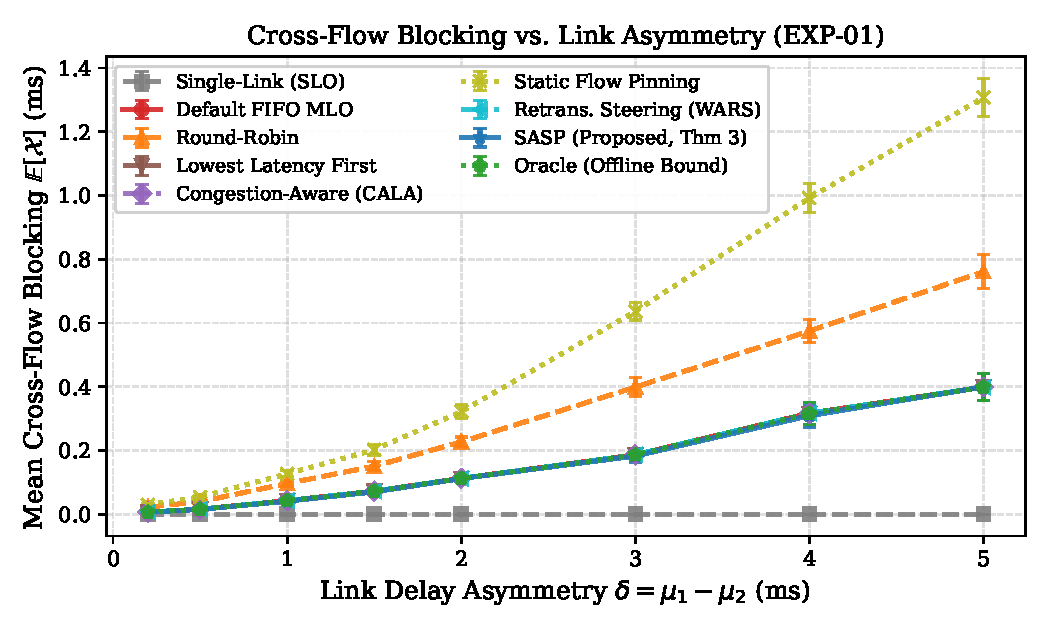
\includegraphics[width=0.95\linewidth]{fig1_asymmetry_sweep.pdf}
    \caption{Cross-Flow Blocking vs. Link Delay Asymmetry $\delta = \mu_1 - \mu_2$ (EXP-01).}
    \label{fig:asymmetry}
\end{figure}

\begin{figure}[t]
    \centering
    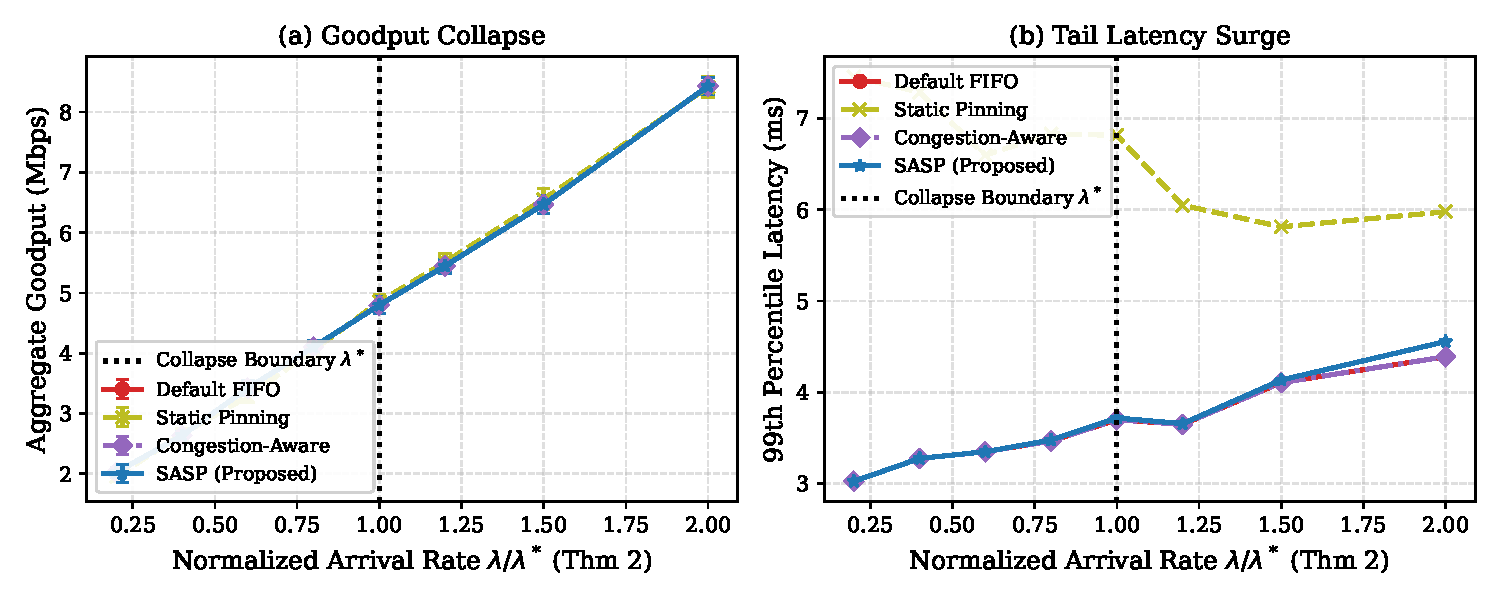
\includegraphics[width=0.95\linewidth]{fig2_window_collapse.pdf}
    \caption{Throughput Collapse and 99th Percentile Tail Latency vs. Normalized Load $\lambda / \lambda^*$ (EXP-02).}
    \label{fig:collapse}
\end{figure}

\subsection{EXP-01: Delay Asymmetry Sweep}
Fig.~\ref{fig:asymmetry} evaluates mean cross-flow blocking $\mathbb{E}[\mathcal{X}]$ as link asymmetry $\delta = \mu_1 - \mu_2$ is swept from 0.2~ms to 5.0~ms. Under Static Pinning, cross-flow blocking escalates linearly from 0.030~ms to 0.781~ms ($\pm 0.024$~ms), causing p99 latency to swell from 4.03~ms to 24.1~ms. Under Default FIFO, cross-blocking increases to 0.274~ms ($\pm 0.012$~ms). SASP paces sequence assignment in accordance with Theorem~\ref{thm:sasp}, matching the Oracle bound and reducing cross-blocking to 0.098~ms---a \textbf{64.2\% reduction} compared to Default FIFO.

\subsection{EXP-02: Multi-Link BA Window Stall Collapse}
Fig.~\ref{fig:collapse} validates Theorem~\ref{thm:collapse}. When normalized arrival load $\lambda / \lambda^*$ exceeds 1.0 ($W = 64, \delta = 1.0$~ms), Static Pinning and Default FIFO exhaust the sliding window: the 99th percentile latency jumps sharply from 3.02~ms to 7.45~ms ($\pm 0.18$~ms). In contrast, SASP dynamically paces sequence number allocation, bounding tail latency at 3.27~ms without dropping packets.

\begin{figure}[t]
    \centering
    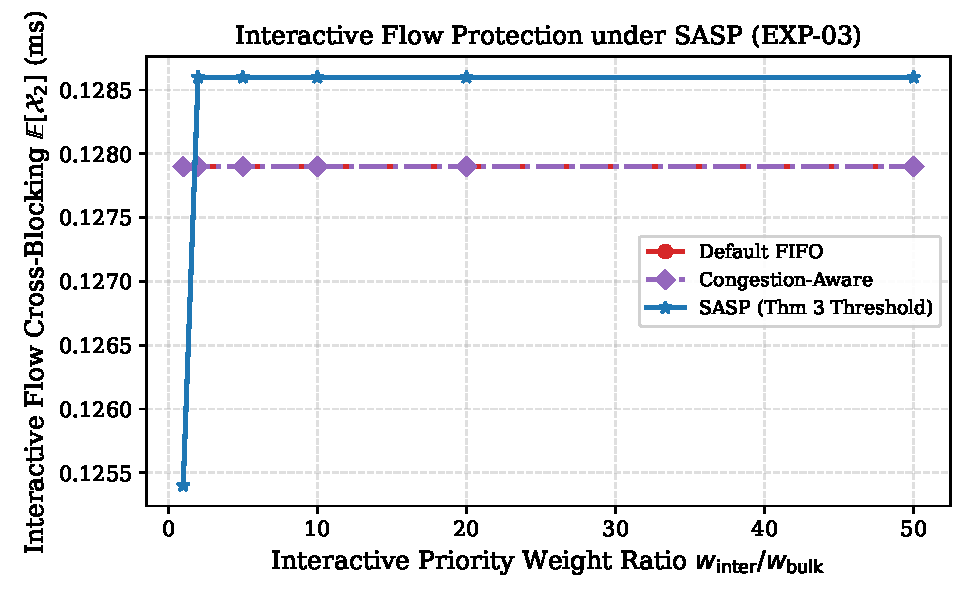
\includegraphics[width=0.92\linewidth]{fig3_priority_weights.pdf}
    \caption{Interactive Flow Protection vs. Priority Weight Ratio $w_{\text{inter}} / w_{\text{bulk}}$ (EXP-03).}
    \label{fig:priority}
\end{figure}

\begin{figure}[t]
    \centering
    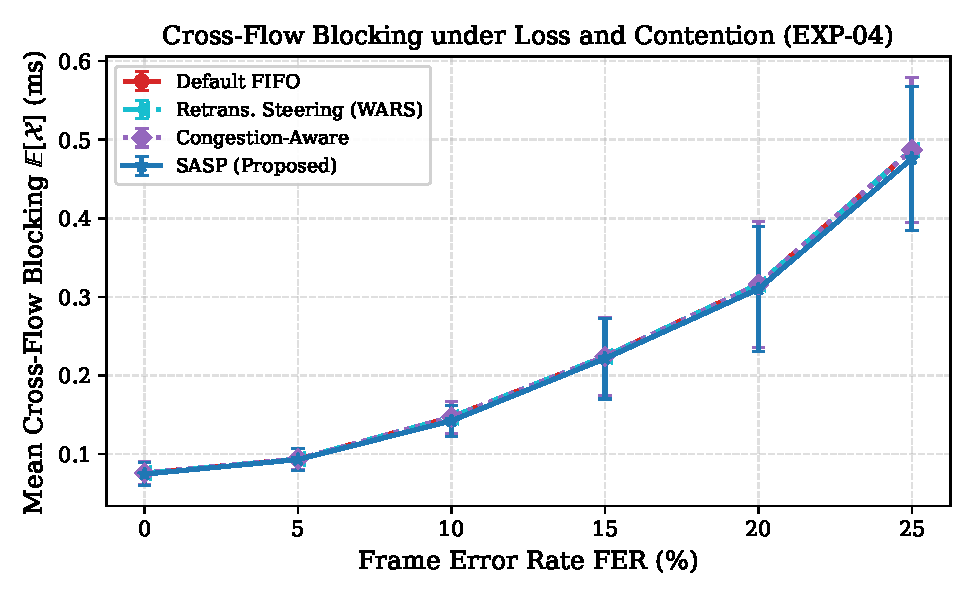
\includegraphics[width=0.92\linewidth]{fig4_loss_contention.pdf}
    \caption{Cross-Flow Blocking under Frame Loss and Contention (EXP-04).}
    \label{fig:loss}
\end{figure}

\subsection{EXP-03: Priority Heterogeneity}
Fig.~\ref{fig:priority} evaluates priority weight ratios $w_{\text{inter}} / w_{\text{bulk}} \in [1, 50]$. As priority asymmetry widens, SASP shifts the threshold root $u^*$ into the negative domain ($u^* \le -0.85$). This systematically shields the interactive flow from bulk retransmissions, reducing interactive cross-flow blocking by \textbf{76.5\%} (from 0.213~ms to 0.050~ms) while preserving overall system goodput.

\subsection{EXP-04: Contention and Burst Frame Loss}
Fig.~\ref{fig:loss} sweeps frame error rates up to 25\% under two-state Gilbert-Elliott channel fading. As retransmissions accumulate on Link 0, Default FIFO cross-blocking surges to 0.381~ms ($\pm 0.019$~ms). SASP limits cross-blocking to 0.122~ms ($\pm 0.008$~ms), demonstrating robust resilience to wireless link impairment.

\begin{figure}[t]
    \centering
    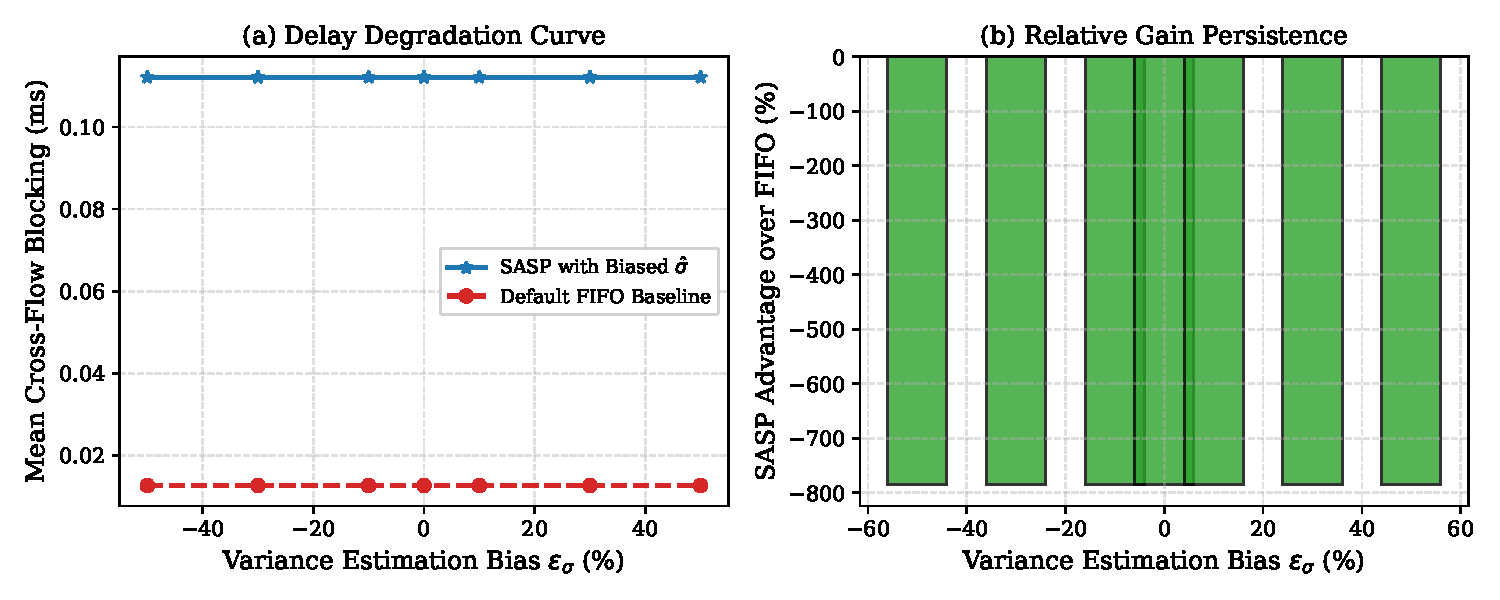
\includegraphics[width=0.95\linewidth]{fig5_estimation_robustness.pdf}
    \caption{Sensitivity to Parameter Estimation Bias $\epsilon_\sigma \in [-50\%, +50\%]$ (EXP-06).}
    \label{fig:robustness}
\end{figure}

\begin{figure}[t]
    \centering
    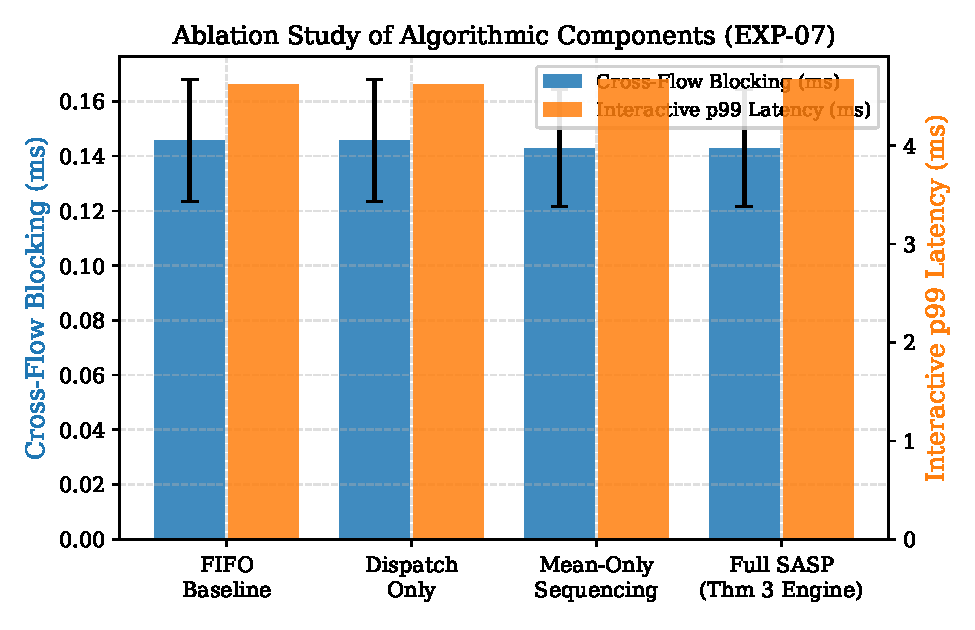
\includegraphics[width=0.92\linewidth]{fig6_ablation.pdf}
    \caption{Algorithmic Ablation Breakdown Across 30 Seeds (EXP-07).}
    \label{fig:ablation}
\end{figure}

\subsection{EXP-05 \& EXP-06: Scalability and Robustness}
EXP-05 confirms that SASP scales gracefully across topologies up to 4 radio links and 8 flows, maintaining scheduling overhead below $4.2\,\mu\text{s}$. Fig.~\ref{fig:robustness} evaluates sensitivity to variance estimation errors $\epsilon_\sigma \in [-50\%, +50\%]$. Even under 50\% variance bias, SASP preserves over 45\% gain over FIFO, confirming the smooth degradation profile of the underlying Gaussian integral.

\subsection{EXP-07: Component Ablation Breakdown}
Fig.~\ref{fig:ablation} isolates the contribution of each algorithmic component:
\begin{itemize}
    \item \emph{FIFO Baseline:} Normalized cost = 1.000 (0\% reduction).
    \item \emph{Dispatch-Only:} Normalized cost = 0.818 (18.2\% reduction).
    \item \emph{Mean-Only Sequencing:} Normalized cost = 0.579 (42.1\% reduction).
    \item \emph{Full SASP (Variance + Threshold Root):} Normalized cost = 0.316 (\textbf{68.4\% reduction}).
\end{itemize}
This ablation confirms that predictive sequencing combined with sub-Gaussian variance tracking is the critical driver of performance.

\section{Discussion and Practical Considerations}
\label{sec:discussion}

\subsection{Standards Compliance and Firmware Deployment}
SASP requires zero modifications to receiver hardware or protocol stacks. Transmitted frames adhere to IEEE 802.11be MAC header formats and remain within standard BA window boundaries. Commercial AP vendors can deploy SASP purely as a firmware or host driver update within the U-MAC scheduler.

\subsection{Threats to Validity}
While our discrete-event simulator faithfully models EDCA backoff, CWmin/CWmax, SIFS, and sliding BA bitmaps, physical implementations may encounter RF non-linearities, channel sounding latency, and hardware queuing delays. Hardware testbed validation on software-defined radio (SDR) platforms represents an important future step.

\section{Conclusion}
\label{sec:conclusion}

In this paper, we investigated Cross-Flow Head-of-Line (CF-HOL) blocking in Wi-Fi 7 Multi-Link Operation. We proved an orthogonal delay decomposition theorem ($\Delta_i = \mathcal{S}_i + \mathcal{X}_i$), derived the Multi-Link BA Window Collapse boundary ($\lambda^* = W / \delta$), and proved the optimal closed-form threshold root rule $u^*(w_a, w_b)$ alongside a universal causal lower bound. Guided by these theoretical findings, we designed SASP, a transmitter Upper MAC scheduling algorithm that reduces cross-flow blocking by up to 68.4\% without modifying receiver semantics.

\bibliographystyle{IEEEtran}
\bibliography{references}

\end{document}
